\documentclass[12pt, a4paper]{book}
% \documentclass{scrbook}   % KOMA-Script Alternative
\usepackage[T1]{fontenc}    % Für korrekten Input und Output mit Sonderzeichen
\usepackage[ngerman]{babel} % Für deutsche Rechtschreibung
\usepackage{appendix}       % Für Anhänge
\usepackage{graphicx}       % Um Bilder einzufügen
\usepackage{lipsum}         % Für Blindtext
\usepackage{booktabs}       % Für feinere Tabellen-Einstellungen
\usepackage[
      colorlinks,
      citecolor=black,
      filecolor=black,
      linkcolor=black,
      urlcolor=black
      ] {hyperref}          % Für klickbare Links in Referenzen
\usepackage{biblatex}       % Für das Literaturverzeichnis
\bibliography{references}   % Einbinden der Referenzliste
\usepackage[Rejne]{fncychap}% Für kreative Kapitelmarker
\usepackage{titling}        % Für Definition einer eigenen Titelseite
\usepackage{xcolor}         % Adding extra colours

% Definitionen

\newcommand{\figref}[1]{Abb.~\ref{#1}}

% Persönliche Angaben

\title{Titel der Arbeit}
\author{Sabrina Patsch}
\date{\today}

% Definition der Titelseite

\renewcommand{\maketitle}{
	\thispagestyle{empty}
	\vspace*{\fill}
	\vspace{20pt}
	\begin{center}
	\Huge \textbf{\textcolor{violet}{\thetitle}} \\
	\vspace{20pt}
    \Large Dissertation
    \normalsize \\
	\vspace{30pt}
	\textsc{Der Miskatonic University \\
    zur \\
    Erlangung des Doktorgrades \\
    \vspace{20pt}
	Dr. rer. mag. \\
    \vspace{20pt}
    
\includegraphics[width=7cm]{images/uni-logo.jpg}\\
	\vspace{20pt}
	vorgelegt von \\
	\vspace{20pt}
	\theauthor \\
	\vspace{20pt}
	aus Miskatonic
	}
	\end{center} \vspace*{\fill}
}

% Inhalt des Dokuments

\begin{document}

\maketitle          % Titelseite

\tableofcontents    % Inhaltsverzeichnis
\listoffigures      % Abbildungsverzeichnis
\listoftables       % Tabellenverzeichnis

% Einbinden der Kapitel

\chapter{Titel des ersten Kapitels}
\label{chapter1}

\section{Erster Abschnitt}

\lipsum[1-2] Dies sehen Sie in \figref{fig:Alice} auf Seite~\pageref{fig:Alice}. Weitere Hinweise finden Sie in \cite{latex-einfuehrung}.

% Siehe dazu auch \cite{latex-einfuehrung} von \ac{sp} aus der \ac{ct}. Also \ac{sp} aus der \ac{ct}.

\begin{figure}[tb]
    \centering
    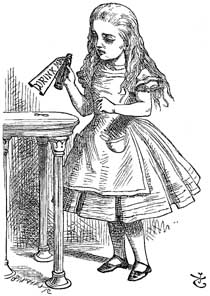
\includegraphics[width=0.5\textwidth]{images/alice.jpg}
    \caption[Alice mit Trinkflasche]{Um den Hals des Fläschchens war ein Zettel gebunden, mit den Worten "Trinke mich!" wunderschön in großen Buchstaben drauf gedruckt.
    \label{fig:Alice}}
\end{figure}

\subsection{Erster Unterabschnitt}

\subsubsection{Erster Unterunterabschnitt}

\lipsum[1-3]

\begin{table}[tb]
    \centering
    \begin{tabular}{ c | c c c }
        \toprule
                & Kaffee & Tee & Bier\\ 
        \midrule
        Morgens & 1 & 2 & 0\\  
        Mittags & 2 & 0 & 0\\ 
        Abends  & 0 & 3 & 1\\ 
        \bottomrule
    \end{tabular}
    \caption[Getränkeübersicht]{Übersicht über die Getränke, die an einem typischen Freitag  getrunken wurden.}
    \label{table:tab1}
\end{table}


\chapter{Titel des zweiten Kapitels}
\label{chapter2}

\lipsum[1-3]

% Einbinden des Anhangs

\begin{appendices}
    \pagenumbering{Roman}
    \chapter{Extra Inhalte}
\label{AppendixA}

\lipsum[4]
\end{appendices}

% Literaturverzeichnis

\phantomsection
\addcontentsline{toc}{chapter}{Literaturverzeichnis}
\printbibliography

\end{document}
